%% LaTeX-Beamer poster template for KIT design
%% by Erik Burger, Christian Hammer
%%
%% version 1.2
%%
%% mostly compatible to KIT corporate design v1.2
%% http://www.uni-karlsruhe.de/download/uka/Gestaltungsrichtlinien_komplett.pdf
%%
%% Problems, bugs and comments to
%% burger@kit.edu

\documentclass{beamer}

%% Fill in the page size here. If the proportions of the fonts
%% are not satisfactory, change the scale parameter
\usepackage[orientation=portrait,size=a1,scale=1.4]{beamerposter}
\usepackage[utf8]{inputenc}
\usepackage{enumitem}
\usepackage{subfigure}
\setitemize{label=\usebeamerfont*{itemize item}%
  \usebeamercolor[fg]{itemize item}
  \usebeamertemplate{itemize item}}
\mode<presentation>{\usetheme{kitposter}}

\title[gr-inspector]{The Inspector (gr-inspector)}
\subtitle{A Signal Analysis Toolbox for GNU Radio}
\author{Sebastian Müller, Karlsruhe Institute of Technology}

\institute{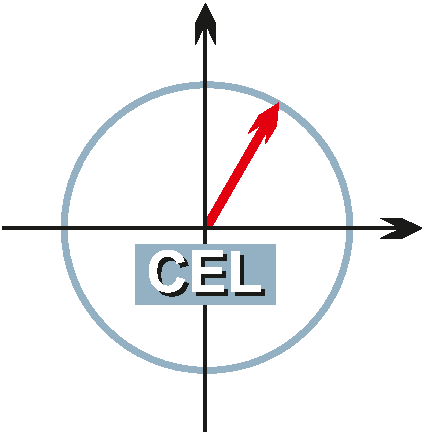
\includegraphics[height=250px]{logos/cel.pdf}\textbf{Communications Engineering Lab}\\[.4em]
Kreuzstr. 11\\[.2em]
76137 Karlsruhe\\[.4em]
\href{http://www.cel.kit.edu}{http://www.cel.kit.edu}}

\begin{document}
% change the following line to "ngerman" for German style date and logos
\selectlanguage{english}

\begin{frame}
  \begin{columns}[t]
    \begin{column}{0.33\textwidth}
      \frametitle{Main}
      \begin{block}{Introduction}
        The Inspector is an out-of-tree module for GNU Radio. The goal was to develop a \textbf{signal analysis toolbox} with the following real-time capabilities:\\[0.5em]
        \begin{itemize}[leftmargin=2.5em]
	        \item Automatic detection of continuous signals
	        %\item Automatic Signal Classification (AMC)
	        \item Automatic signal extraction
          \item OFDM parameter estimation and synchronization
	        \item GUI feedback
        \end{itemize}
        \vspace{0.5em}
        This project was initiated as a Google Summer of Code project and developed in cooperation with the Communications Engineering Lab of the Karlsruhe Institue of Technology.
      \end{block}
      \begin{block}{Components}
\textbf{Signal Detector}
is able to perform energy detection on a continuous input signal.\\[0.5em]

\textbf{Inspector GUI}
visualizes the detected signal edges. Users can select signals manually and feed-back results from analysis blocks.\\[0.5em]

\textbf{Signal Separator}
uses FIR filters for every detected/selected input signal to mix, filter and decimate this signal out of the input spectrum. Output is a message of vectors with samples of all signals.\\[0.5em]

\textbf{Signal Extractor}
passes one signal from the Separator output as complex stream. The input samples can be resampled to satisfy a constant output sample rate.\\[0.5em]

\textbf{OFDM Estimator}
is able to estimate the OFDM parameters subcarrier spacing, symbol time, FFT lenght and CP length.\\[0.5em]

\textbf{OFDM Synchronizer}
performs a frequency synchronization of the OFDM signal and stream tags are inserted at OFDM symbol beginnings.\\[0.5em]

\textbf{AMC Functionality}
is available through additional blocks developed by Christopher Richardson (ESA SOCIS student).

\vspace{1.5em}
      \end{block}
    \end{column}
    \begin{column}{0.01\textwidth}
    \end{column}
    \begin{column}{0.66\textwidth}
      \begin{block}{Flowgraph}
        The toolbox was developed with the following main flowgraph in mind.
        \begin{figure}
          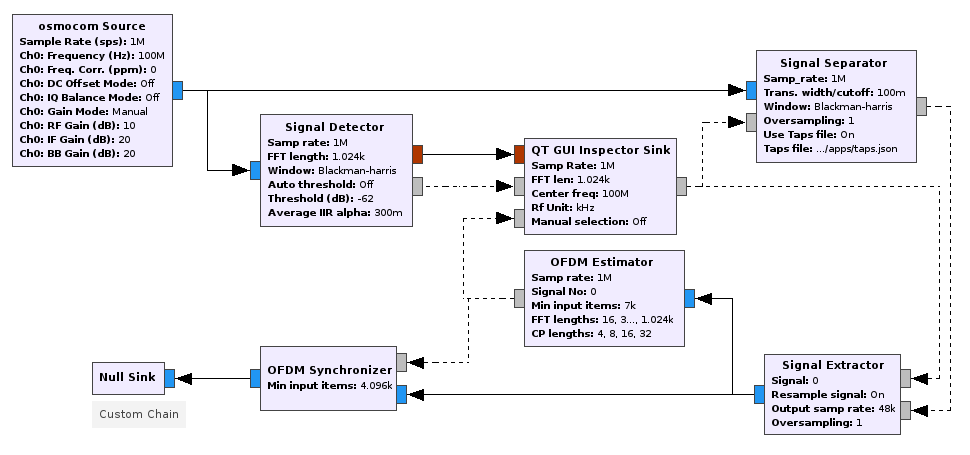
\includegraphics[width=\textwidth]{figures/flowgraph}
        \end{figure}
        \begin{itemize}
          \item Signal Extractor block assures the possibility to add \textbf{custom chains} for each signal 
          \item Analysis blocks can \textbf{feedback results} to GUI block
        \end{itemize}
      \end{block}
      \begin{block}{GUI}
      \begin{figure}
        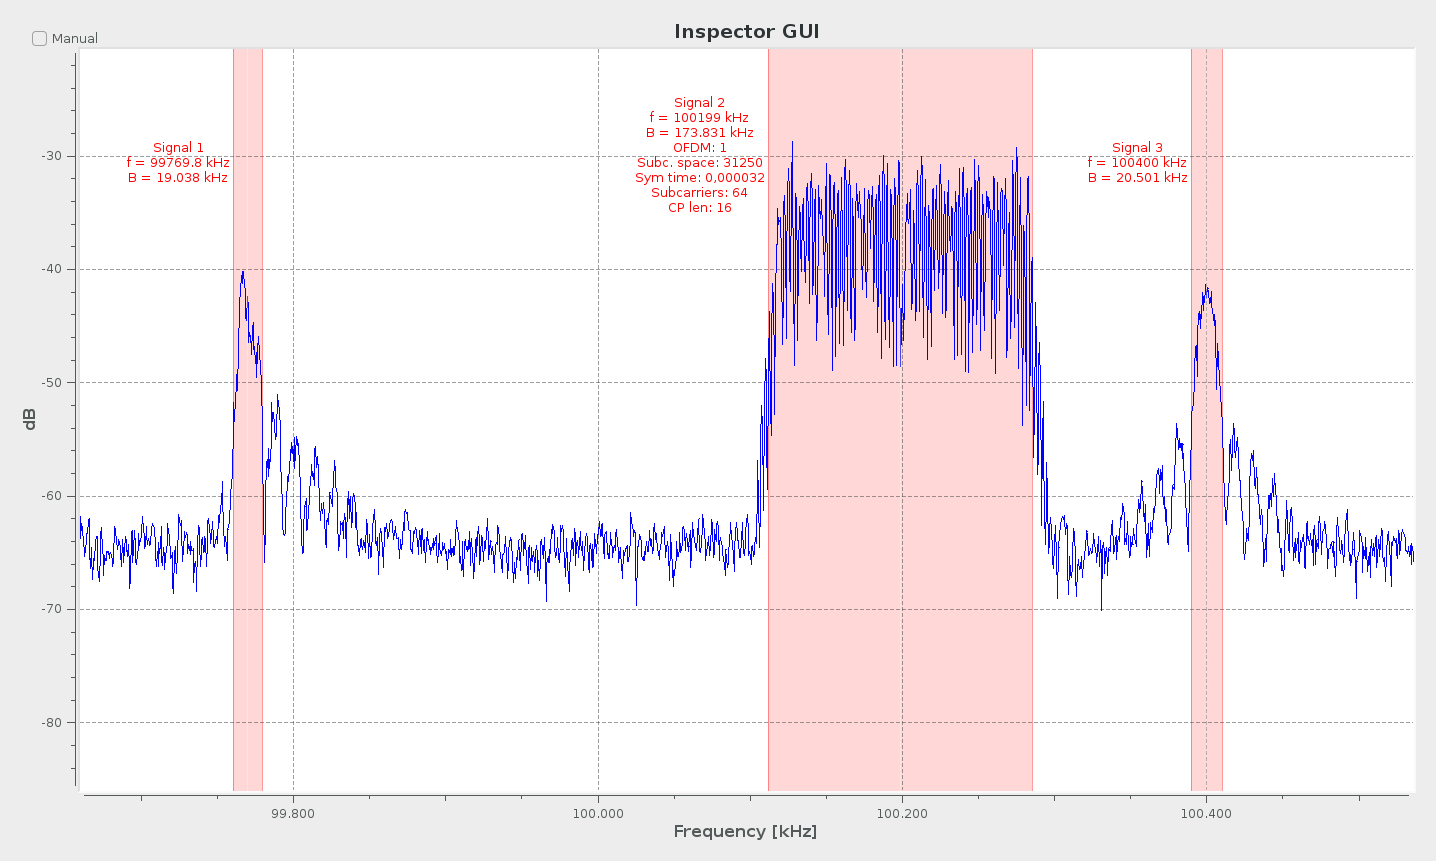
\includegraphics[width=\textwidth]{figures/gui.png}
      \end{figure}
      \begin{itemize}
        \item Displays input spectrum with \textbf{markers for detected signals}
        \item \textbf{Info text} next to each signal (center frequency, bandwidth and analysis results)
        \item Each signal can be filtered and processed in \textbf{own chain(s)}
        \item Signals can be selected manually
      \end{itemize}
      \end{block}
    \end{column}
  \end{columns}
  \begin{columns}[t]
  	\begin{column}{0.66\textwidth}
  		\begin{block}{Applications}
  			\begin{columns}
        \begin{column}{0.45\textwidth}
        \begin{itemize}
          \item Spectrum monitoring
          \item Explore real-world signals
          \item Access to radio for beginners
        \end{itemize}
        \end{column}
        \begin{column}{0.45\textwidth}
         \begin{itemize}
          \item Live (FM) demodulation
          \item Batch processing of signals
        \end{itemize}
        \end{column}
        \end{columns}
  		\end{block}
  	\end{column}
  	\begin{column}{0.01\textwidth}
  	\end{column}
  	\begin{column}{0.33\textwidth}
  		\begin{block}{Contact}
  			Sebastian Müller

  			Karlsruhe Intitute of Technology

  			gsenpo@gmail.com
  			\vspace{0.3em}
  		\end{block}
  	\end{column}
  \end{columns}
\end{frame}
\end{document}
